% !TeX document-id = {e910d311-1b9f-412a-806f-acb4afe000c4}
% !TeX TXS-program:compile = txs:///pdflatex/[--shell-escape] | txs:///biber | txs:///pdflatex/[--shell-escape]
\documentclass[3p,times,a4paper,twocolumn,authoryear]{elsarticle} %authoryear

%% Fix so biblatex works instead of natbib
\makeatletter
\let\c@author\relax
\makeatother
\let\bibhang\relax
\let\citename\relax
\let\bibfont\relax
\let\Citeauthor\relax
\expandafter\let\csname ver@natbib.sty\endcsname\relax

%% Fix headers and footers
\makeatletter
\def\ps@pprintTitle{%
	\let\@oddhead\@empty
	\let\@evenhead\@empty
	\def\@oddfoot{\centerline{\thepage}}%
	\let\@evenfoot\@oddfoot}
\makeatother

%% Load some packages and stuff
%\usepackage[backend=biber,style=numeric, defernumbers=true, sorting=ynt,maxbibnames=4,maxcitenames=4]{biblatex}
%% Library and stuff
\usepackage[style=numeric,sortcites=true,sorting=ynt,backend=biber]{biblatex}
%% biblatex med apa-style. Det vivill ha
\DeclareLanguageMapping{american}{american-apa} %% Vi vill ha svensk apa
\bibliography{../bibliography/reference}

\usepackage[T1]{fontenc}
\usepackage[spanish]{babel}
\usepackage{pifont}
\usepackage{geometry}
\usepackage[svgnames]{xcolor}
\usepackage{graphicx}
\usepackage{sagetex}
\usepackage{minted}
\usepackage{float}
\usepackage{tkz-graph}
\usepackage{txfonts}
\usepackage{amsmath,amsthm}
\theoremstyle{definition}
\usepackage{bm}
\usepackage[colorlinks=true,urlcolor=blue,linkcolor=black,anchorcolor=black,citecolor=black]{hyperref}
\hypersetup{pdfinfo={
		Title={El teorema de los cuatro colores},
		Author={Grupo Nº6},
		Keywords={teorema de los cuatro colores, cadena de Kempe, grafos planares, coloración de mapas},
		Subject={Introducción a la matemática discreta},
		Producer={TeXstudio 2.12.8},
		Creator={pdfTeX Version 3.14159265 TeX Live 2018 Debian}
}}


\usepackage{etoolbox}
\AtBeginDocument{%
	%\patchcmd{<cmd>}{<search>}{<replace>}{<success>}{<failure>}
	%\patchcmd{\ps@pprintTitle}% <cmd>
	%{Preprint submitted}% <search>
	%{To be submitted}% <replace>
	%{}{}% <succes><failure>
	\patchcmd{\MaketitleBox}{\vspace*{-20pt}\fi}{\fi}{}{}%
	\patchcmd{\abstract}{Abstract}{Resumen}{}{}
	\patchcmd{\keyword}{Keywords}{Palabras clave}{}{}
}

%\makeatletter
%\patchcmd{\ps@pprintTitle}{\footnotesize\itshape
%	Preprint submitted to \ifx\@journal\@empty Elsevier
%	\else\@journal\fi\hfill\today}{\relax}{}{}
%\makeatother

\makeatletter
\def\printFirstPageNotes{%
	\iflongmktitle
	\let\columnwidth=\textwidth\fi
	\ifx\@tnotes\@empty\else\@tnotes\fi
	\ifx\@nonumnotes\@empty\else\@nonumnotes\fi
	\ifx\@cornotes\@empty\else\@cornotes\fi
	\ifx\@elseads\@empty\relax\else
	\let\thefootnote\relax
	\footnotetext{\ifnum\theead=1\relax
		\textit{Correo electrónico:\space}\else
		\textit{Correos electrónicos:\space}\fi
		\@elseads}\fi
	\ifx\@elsuads\@empty\relax\else
	\let\thefootnote\relax
	\footnotetext{\textit{Sitio web:\space}%
		\@elsuads}\fi
	\ifx\@fnotes\@empty\else\@fnotes\fi
	\iflongmktitle\if@twocolumn
	\let\columnwidth=\Columnwidth\fi\fi
}
\makeatother

%% `Elsevier LaTeX' style
%\bibliographystyle{elsarticle-num}
\renewcommand{\spanishcontentsname}{Tabla de contenidos}
\renewcommand{\spanishfigurename}{Fig.}
\renewcommand{\listingscaption}{Programa}
%\newcommand{\MVAt}{{\usefont{U}{mvs}{m}{n}\symbol{`@}}}
\newtheorem{definition}{Definición}
\newtheorem{example}{Ejemplo}
\newtheorem{theorem}{Teorema}

\graphicspath{{../images/}}

\usepackage{ecrc}

\volume{06}

\firstpage{1}

\runauth{Grupo N$^{\circ}6$}%C. Aznarán et al.

\jnltitlelogo{\large Annals of Discrete Mathematics FC-UNI}

\begin{document}

\begin{abstract}

En este trabajo, estudiamos las propiedades de los grafos duales, los números cromáticos y los polinomios cromáticos de los grafos planares para la prueba del teorema de los cuatro colores. Además, mostraremos la interrelación entre este tipo de grafos. Al haber presentado las definiciones establecidas para los grafos duales, se buscará una representación análoga para los mapas conexos. También se mostrará el \emph{algoritmo de las cadenas de Kempe}, el cual es famoso por ser la primera ``demostración del teorema de cuatro colores''. Asimismo, se evaluará este algoritmo para los grafos de Errera, Kittell, Soifer, Fristsch y Poussin, los cuales son contraejemplos de su prueba que data desde 1921. Se mencionará la idea clave \citeauthor{birkhoff} publicado en \cite{birkhoff}. También, con el uso un CAS (Sistema algebraico computacional) Sage en el cual se hallará el número cromático y sus polinomios cromáticos respectivamente. Finalmente se mostrarán algunas aplicaciones con la resolución del Sudoku y un programa llamado \texttt{TEOCOLOR}.
\\[1mm]
\textcopyright\ Science Department National University of Engineering Publishers Inc. All rights reserved.

\end{abstract}

\begin{keyword}
teorema de los cuatro colores \sep cadena de Kempe\sep grafos planares\sep coloración de mapas
\end{keyword}

\begin{frontmatter}

\title{El teorema de los cuatro colores\tnoteref{t1,t2}}
\tnotetext[t1]{Este documento es un esfuerzo colaborativo.}
\tnotetext[t2]{Este informe está disponible en \href{https://github.com/carlosal1015/4colores}{GitHub}.}

%% Group authors per affiliation:
\author[1,3]{C.~Aznarán Laos\corref{correspondingauthor}}
\ead{caznaranl@uni.pe}

\ead[url]{www.blogdeoromion.pe.hu}

\author[1,3]{F.~Cruz Ordoñez\corref{mycorrespondingauthor}}
\ead{fransscruz18@gmail.com}

\author[2,3]{J.~Navío Torres\corref{mycorrespondingauthor}}
\ead{jnavio@uni.pe}

%% or include affiliations in footnotes:
\author[1,3]{G.~Quiroz Gómez\corref{mycorrespondingauthor}}
\ead{ge\_qg\_25@hotmail.com}

\address[1]{Facultad de Ciencias - Escuela Profesional de Ciencia de la Computación}
\address[2]{Facultad de Ciencias - Escuela Profesional de Matemática}
\address[3]{Universidad Nacional de Ingeniería,	Av. Túpac Amaru 210, Rímac, Lima 25, Perú}

\end{frontmatter}

\tableofcontents

\section{Introducción}\label{sec:1}

En la sección~\ref{sec:1}, recordaremos los eventos más importantes en la historia del teorema de los cuatro colores. En la sección~\ref{sec:2} damos las definiciones de los grafos planares y los grafos duales. La conexión entre los grafos planares y los mapas conexas viene dada por la \emph{Fórmula de Euler}. La coloración, el número cromático y el polinomio cromático se definen en la sección~\ref{sec:2}. Con estos preparativos, en la sección~\ref{sec:3} demostramos que el número cromático es el menor índice de un número cromático y presentaremos el algoritmo de las cadenas de Kempe. Asimismo, en la sección~\ref{sec:3} se mostrará los contraejemplos de su prueba. Véase~\cite{errera} para más detalles. Posteriormente revisamos las definiciones sobre el método de descarga y encontraremos la noción dada por \citeauthor{birkhoff} sobre configuraciones reducibles publicado en \cite{birkhoff}. En la subsección~\ref{sec:3.3} utilizaremos el Sistema algebraico computarizado de código abierto Sage\TeX{} para ilustrar algunos ejemplos visto en la sección \ref{sec:2} tales como coloración de grafos, número cromático y polinomio cromático. Finalmente, en la Sección \ref{sec:4}, damos algunas aplicaciones para el juego del sudoku y el programa \texttt{TEOCOLOR}.

%El propósito de este reporte es mostrar las técnicas matemáticas o \emph{algoritmos} utilizados en las demostraciones. Asimismo se mostrará algunos cálculos numéricos usando el CAS Sage y se mostrará ejemplos con las definiciones empleadas. Se invita a los matemáticos a que revisen la bibliografía citada.

\subsection{¿Qué es una conjetura?}\label{sec:1.1}
Una conjetura es una afirmación que se toma por verídica, pero que no ha sido probada o refutada hasta la fecha. Cuando una conjetura es demostrada ésta recién toma el carácter de Teorema.

\subsection{Teorema de  los 4 colores}\label{sec:1.2}

El teorema de los 4 colores fue enunciado por primera vez como una conjetura en el año de 1852 por el botánico y abogado Francis Guthrie después de haber coloreado un mapa complejo de las calles de Inglaterra con tan solo 4 colores.

\noindent El teorema tiene ya más de 100 años entre nosotros, pero tuvieron que llegar \citeauthor{appel} con la demostración definitiva en 1976, y gracias a la capacidad de procesamiento de los ordenadores, lograron comprobar una colección de aproximadamente 1900 mapas básicos que ellos mismos habían diseñado y que constataron así la validez del Teorema, esto fue algo polémico ya que nunca se había usado los ordenadores para hacer una demostración matemática formal.

\subsection{¿Qué dice el Teorema?}\label{sec:1.3}
El teorema nos dice que cualquier mapa conexo , con cualquier número de regiones y con cualquier forma puede ser pintado con solo 4 colores de tal forma que dos regiones vecinas,contiguas o adyacentes no presenten el mismo color. Un mapa conexo se puede ver como un grafo planar en el cual sus ramas serán las porciones de frontera

\subsection{El problema de los cuatro colores}\label{sec:1.4}

En 1976, \citeauthor{appel} lograron un gran avance al establecer cuidadosamente el \emph{Teorema de los cuatro colores}. Su prueba se basa en estudiar una gran cantidad de casos para los cuales se requiere una búsqueda asistida por computadora por horas. En 1997, el fue reprobado con menos necesidad de verificación por computadora por \citeauthor{Robin}. Sin embargo, \citeauthor{kempe} en 1879 diseñó un método que se conoce como las \emph{cadenas de Kempe} para su prueba errada del teorema, enunciaremos las definiciones y mostraremos ejemplos, en particular, los grafos de Errera, Kittell, 

\subsection{Algunas fechas importantes}\label{sec:1.5}

A continuación, se listan algunos de los eventos más importantes desde su creación hasta el desenlace a fines del siglo XX.

\begin{enumerate}
	
	\item[{\color{DarkBlue}1852}] Francis Guthrie plantea el problema a su hermano Frederick y este a Augustus de Morgan.
	
	\item[{\color{DarkBlue}1878}] Arthur Cayley publica el enunciado de la conjetura.
	
	\item[{\color{DarkBlue}1879}] Sir Alfred Bray Kempe publica su demostración.
	
	\item[{\color{DarkBlue}1890}] Percy Heawood descubre un error insalvable en la prueba dada por Kempe.
	
	\item[{\color{DarkBlue}1913}] George Birkhoff introduce la noción de configuración reducible.
	
	\item[{\color{DarkBlue}1960}] Se introduce el llamado método de descarga.
	
	\item[{\color{DarkBlue}1969}] Avances de Heinrich Heesch en reducibilidad y obtención de conjuntos inevitables de configuraciones.
	
	\item[{\color{DarkBlue}1976}] \citeauthor{appel} prueban con ayuda de un ordenador que sus 1.482 configuraciones son reducibles (50 días de cálculo).
	
	\item[{\color{DarkBlue}1996}] \citeauthor{robertson} mejoran la demostración con ayuda de ordenador (solo 633 configuraciones) y automatizan la prueba de la inevitabilidad.
	
	\item[{\color{DarkBlue}2000}] Ashay Dharwadker da otra prueba del teorema de los 4 colores, no basada en ideas previas, utilizando teoría de grupos, teoría de sistemas de Steiner y correspondencias de Hall.
	
	\item[{\color{DarkBlue}2004}] Ibrahim Cahit, dice haber demostrado la conjetura, usando el nuevo concepto de cadenas espirales, sin ordenador.

\end{enumerate}

\section{Definiciones previas}\label{sec:2}

\subsection{Mapa conexo}\label{sec:2.1}
Un mapa conexo se puede ver como un grafo planar en el cual las porciones de frontra son las ramas del grafo.

\begin{figure}[H]
	\centering
	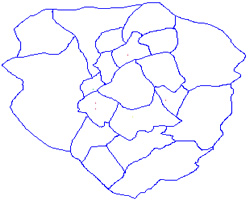
\includegraphics[width=4cm]{conexo}
	\caption{Mapa Conexo}
\end{figure}    

Si $G$ es un grafo sin lazos, entonces $G$ es \textbf{$\bm{k}$-coloreable} si podemos asignar uno de $k$ colores a cada vértices de manera que vértices adyacentes tengas diferentes colores. Si $G$ es $k$-coloreable, pero no $(k-1)$- coloreable, diremos que $G$ es \textbf{$\bm{k}$-cromático}, o que el \textbf{número cromático} de $G$ es $k$, y lo denotamos por $\chi(G)=k$. Por ejemplo, la Figura~\ref{fig:1.1} muestra un grafo para el cual $\chi(G)=4$; los colores son dentados por las letras griegas. Es por lo tanto $k$-coloreable si $k>4$. Deberíamos asumir que todos los grafos aquí son simples, ya que los bordes múltiples son irrelevantes para nuestra discusión. También asumiremos que están conectados.

Es claro que $\chi(K_n)=n$, y así, existen grafos con un número cromático grande y arbitrario. En el otro extremo de la escala, $\chi(G)=1$ si y solo si $G$ es el grafo nulo, y $\chi(G)=2$ si y solo si $G$ es un grafo bipartito no nulo. Note que cualquier árbol es $2$-coloreable, así como cualquier ciclo con un número par de vér

\begin{figure}[H]
\centering
\scalebox{0.6}{\begin{tikzpicture}
	\SetGraphUnit{4}
	\GraphInit[vstyle=Classic]
	%\SetVertexNoLabel
	\Vertex[L={\LARGE$\alpha$}, Lpos=180]{a}
	\EA[L={\LARGE$\gamma$}](a){b}
	\NOEA[L={\LARGE$\beta$},Lpos=90](b){c}
	\SOEA[L={\LARGE$\delta$}, Lpos=-90](b){d}
	\EA[unit=7, L={\LARGE$\alpha$}](b){e}
	\Edges(d,a,b,c,e,d,c,c,a,b,d)
\end{tikzpicture}}
\caption{Grafo $G$}\label{fig:1.1}
\end{figure}

\begin{definition}[Grafo planar]

Un dibujo de un grafo $G=(V,E)$ es una aplicación que a cada vértice $v$ del grafo $G$ le asigna un punto $b(v)$ del plano, y a cada rama $e=\{v,v^{\prime}\}\in E$, le asigna un arco $\alpha(e)$ del plano con $b(v)$ y $b(v^{\prime})$ como puntos finales. Suponemos que la aplicación $b$ es inyectiva (vértices diferentes tienen asignados distintos puntos del plano), y un punto de la forma $b(v)$ no está en ninguno de los arcos $\alpha(e)$ excepto si es un punto final de este arco. Un grafo junto con alguno de sus dibujos se llama grafo topológico.

\end{definition}

\begin{theorem}[Teorema de Kuratowski]

Un grafo $G$ es planar si y solo si no tiene ningún subgrafo isomorfo a una subdivisión de $K_{3,3}$ o una subdivisión de $K_5$.

\end{theorem}

\begin{definition}[Mapa conexo]

Un mapa es conexo\footnote{De una sola pieza.} y cada una de sus regiones también es conexa.

\end{definition}

\begin{definition}[Número cromático]

Sea $G=(V,E)$ un grafo y sea $k$ un número natural. Una aplicación $c\colon V\to \{1,2,\ldots k\}$ se llama \emph{\color{DarkBlue}coloración del grafo} $G$ si $c(x)\neq c(y)$ se cumple para cada rama $\{x,y\}\in E$. \linebreak El \emph{\color{DarkBlue}número cromático} de $G$, denotado por $\chi(G)$, es el \emph{\color{red}mínimo valor} de $k$ para el cual existe una coloración $c\colon V(G)\to\{1,2\ldots,k\}$.

\end{definition}

\begin{definition}[Grafo Dual]

Sea $G=(V,E)$ un grafo planar con un dibujo planar fijo. Denotamos por $\mathcal{F}$ el conjunto de caras de $G$. Definimos un grafo, con posibles lazos y ramas múltiples, como $(\mathcal{F},E,\varepsilon)$, donde $\varepsilon$ se define como $\varepsilon(e)=\{F_i,F_j\}$ siempre que la rama $e$ sea una frontera común de las caras $F_i$ y $F_j$.

Este grafo $\left(\mathcal{F},E,\varepsilon\right)$ se le llama el dual de $G$ y se denota por $G^{\ast}$.
	
\end{definition}

\begin{example}[Grafos Duales]

Para construir una gráfica dual de un grafo plano $G$ se debe colocar un vértice dentro de cada región de $G$ e incluir la región infinita de $G$. Para cada arista compartida por las $2$ regiones, se debe dibujar una arista que conecte a los vértices dentro de estas regiones y para cada arista que se recorre $2$ veces en el camino cerrado alrededor de las aristas de una región se dibuja un lazo en el vértice de la región.

\end{example}

\begin{figure}[H]
\centering
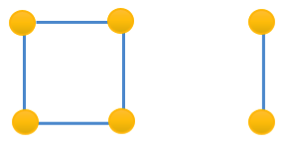
\includegraphics[width=6cm]{example1}
\caption{Grafo $G$.}
\end{figure}

\begin{figure}[H]
	\centering
	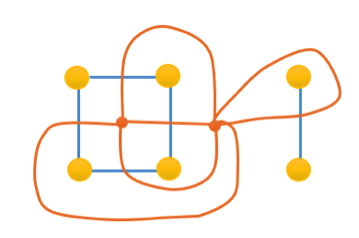
\includegraphics[width=6cm]{example2}
	\caption{Grafo $G$ y su dual $G^{\ast}$.}
\end{figure}

\begin{figure}[H]
	\centering
	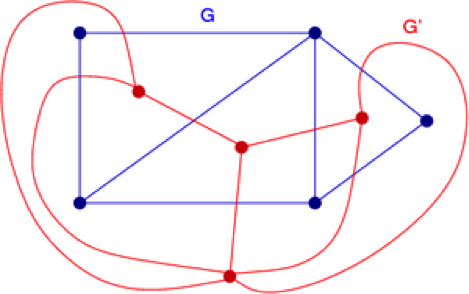
\includegraphics[width=6cm]{example3}
	\caption{Grafo $G$.}
\end{figure}

\begin{definition}[Polinomio cromático]

Sea $G=(V,E)$ un grafo planar y $P(G,k)$ el número de vértices coloreados.
El polinomio cromático cuenta el número de maneras que puede ser coloreado un grafo usando no más de número dado de colores.

\end{definition}

\section{El ``camino'' hacia la demostración}\label{sec:3}

\subsection{La formulación de la conjetura}\label{sec:3.1}

\subsection{La primera ``demostración'': las cadenas de Kempe}\label{sec:3.2}

\begin{definition}[Cadenas de Kempe]
	
	Suponga que un mapa $M$ es coloreado por los colores $a, b, c$ y $d$, seleccione un par de ellos, como $a$ y $b$. Considere cualquier región coloreada en uno de esos pares de colores juntos con todas las regiones de esos colores, adyacente o conexa por un conjunto de regiones en los dos colores. Tal conjunto de regiones será llamado una \emph{cadena} $a,b$. Obviamente, la misma cadena $a,b$ es definida por cualquier región en la cadena.
	
	Una propiedad fundamental de la cadena es que si los dos colores sobre las regiones de una cadena simple, o de cualquier conjunto de esas cadenas de los mismos colores, todas intercambiadas, una nueva coloración de mapas resulta
	
\end{definition}

\begin{definition}[Cadena de Kempe]

Sea $G$ un grafo planar cuyos vértices han sido coloreados apropiadamente y suponga $v\in V(G)$ es coloreado $C_1$. Definimos la \emph{cadena de Kempe} $C_1C_2$ que contiene a $v$ para ser el componente conexa maximal de $G$ que
	
\begin{enumerate}%[label=\arabic*]

	\item Contiene a $v$, y

	\item Contenga solo vértices que son coloreados con elementos desde $(C_1C_2)$.

\end{enumerate}
	
\end{definition}

\subsection{Heawood y el error fatal de \citeauthor{kempe}}\label{sec:3.3}

\begin{figure}[H]
	\centering
	\scalebox{.3}{\begin{tikzpicture}
	\SetGraphUnit{2}
	\GraphInit[vstyle=Classic]
	\SetVertexNoLabel
	\foreach \X/\Y [count=\Z] in {4/ 13, 4/ 6, -0.2/ 5, 2/ 2.2, -6/ -1, 6/ 2.2, 
	9.5/ 1.6, 2.7/ 5, 4.8/ 7.8, 4/ 10.4, -1.5/ 1.6, 14/ -1, 4/ 3.6, 
	5.3/ 5, 3.2/ 7.8, 4/ 0.3, 8.1/ 5}
	{\Vertex[x=\X,y=\Y]{v\Z}}
	\Edges(v2,v8,v13,v14,v2)
	\Edges(v5,v12,v16,v5)
    \Edges(v5,v11,v16,v7,v12)
	\Edges(v11,v4,v16,v6,v7)
	\Edges(v4,v8,v15,v10,v9,v14,v6)
	\Edges(v4,v13,v6,v4)
	\Edges(v13,v2,v15,v9,v2)
	\Edges(v3,v10,v17)
	\Edges(v11,v15,v3)
	\Edges(v7,v9,v17)
	\Edges(v5,v3,v11)
	\Edges(v12,v17,v7)
	\Edges(v5,v1,v12)
	\Edges(v3,v1,v17)
	\Edges(v1,v10)
	\Edges(v11,v8)
	\Edges(v7,v14)
\end{tikzpicture}}
	\caption{Grafo de Errera.}
\end{figure}

\begin{figure}[H]
	\centering
	\scalebox{.25}{\begin{tikzpicture}
	\SetGraphUnit{2}
	\GraphInit[vstyle=Classic]
	\SetVertexNoLabel
	\foreach \X/\Y [count=\Z] in {10.5/ 3, 22/ 0, 10/18, 18/ 2.5, 5/ 3,
		11.7/ 5.6, 1.8/ 1.5, 14/ 7, 7.9/ 9, 7.5/ 6, 12.8/ 1, 9/ 13,
		9.5/ 6, 15/ 4, 11/ 13, 6.5/ 10, 7/ 1.8, -1/ 0, 9.5/ 9,
		13.5/ 10.5, 5.7/ 6.5, 12/ 8.5, 8/ 3.5}
	{\Vertex[x=\X,y=\Y]{v\Z}}
	\Edges(v18,v2,v3,v18)
	\Edges(v7,v16,v12,v15,v20,v4,v11,v17,v7)
	\Edges(v18,v7,v21,v16,v9,v12,v19,v9,v10,v21,v5,v7)
	\Edges(v18,v16,v3,v12,v22,v6,v13,v19,v10,v13,v23,v10,v5,v17,v23,v5)
	\Edges(v21,v9)
	\Edges(v13,v6,v14,v4)
	\Edges(v2,v11,v18)
	\Edges(v11,v1,v17)
	\Edges(v1,v23)
	\Edges(v2,v4,v8,v20,v3)
	\Edges(v14,v8,v22,v15,v8)
	\Edges(v14,v22)
	\Edges(v3,v15)
	\Edges(v12,v6)
	\Edges(v19,v6)
	\Edges(v13,v1,v6,v11,v14)
	\Edges(v18,v17)
	\Edges(v20,v2)
\end{tikzpicture}}
	\caption{Grafo de Kittell.}
\end{figure}

\begin{figure}[H]
	\centering
	\scalebox{0.6}{\begin{tikzpicture}[scale=2]
	\SetGraphUnit{2}
	\GraphInit[vstyle=Classic]
	\SetVertexNoLabel
	\foreach \X/\Y [count=\Z] in {5 /0, 2.5/ 2.35, 0/ 0, 3.2/ 3, 1.8/ 1.7, 3.2/ 1.7,
		1.4/ 0.6, 1.8/ 3, 2.5/ 1.05}
	{\Vertex[x=\X,y=\Y]{v\Z}}
	\Edges(v3,v8,v4,v2,v8,v5,v3,v7,v5,v9,v2,v6,v9,v7,v1,v9)
	\Edges(v1,v6,v4,v1)
	\Edges(v5,v2)
	\Edges(v3,v1)
\end{tikzpicture}}
	\caption{Grafo de Soifer.}
\end{figure}

\begin{figure}[H]
	\centering
	\scalebox{0.45}{\begin{tikzpicture}[scale=6]
	\SetGraphUnit{2}
	\GraphInit[vstyle=Classic]
	\SetVertexNoLabel
	\foreach \X/\Y [count=\Z] in {0.866/ -0.5, 0/ 1, 0.263/ -0.235, 0.188/ 0.0294, -0.866/ -0.5, 0/ -0.323,  -0.263/ -0.235, -0.188/ 0.029, 0/-0.147
	}
	{\Vertex[x=\X,y=\Y]{v\Z}}
	\Edges(v5,v2,v1,v5,v6,v1)
	\Edges(v5,v7,v9,v4,v3,v6,v7,v3,v9,v8,v7)	
	\Edges(v2,v9)
	\Edges(v5,v8,v2,v4,v1,v3)
\end{tikzpicture}}
	\caption{Grafo de Fritsch.}
\end{figure}

\begin{figure}[H]
	\centering
	\scalebox{0.6}{\begin{tikzpicture}[scale=6.5]
	\SetGraphUnit{2}
	\GraphInit[vstyle=Classic]
	\SetVertexNoLabel
	\foreach \X/\Y [count=\Z] in {2.21/ 5.19, 2.19/ 5.4, 2.27/ 5.28, 1.98/ 5.57,  2.42/ 5.54, 2.11/ 5.28, 2.19/ 5.77, 1.61/ 5.07, 2.32/ 5.44, 2.07/ 5.44, 2.85/ 5.07, 2.61/ 5.19, 1.86/ 5.15, 2.19/ 5.53, 2.19/ 6.02}
	{\Vertex[x=\X,y=\Y]{v\Z}}
	\Edges(v8,v15,v11,v8,v13,v4,v7,v5,v12,v1,v13)
	\Edges(v11,v13)
	\Edges(v11,v1)
	\Edges(v11,v12)
	\Edges(v8,v4)
	\Edges(v4,v15)
	\Edges(v15,v7,v14,v4,v10,v13,v6,v1,v3)
	\Edges(v12,v3,v6,v10,v14,v9,v3,v2)
	\Edges(v2,v6)
	\Edges(v2,v10)
	\Edges(v2,v14)
	\Edges(v2,v9,v12)
	\Edges(v7,v9)
	\Edges(v7,v12)
	\Edges(v15,v5,v11)
\end{tikzpicture}}
	\caption{Grafo de Poussin.}
\end{figure}

\begin{listing}[H]
	\inputminted{python}{../code/errera.sage}
	\caption{Programa \texttt{errera.sage}}
\end{listing}


\subsection{Idea clave: la reducibilidad de mapas de \citeauthor{birkhoff}}\label{sec:3.4}

\subsection{El método de descarga de \citeauthor{appel}}\label{sec:3.5}

\section{Aplicaciones}\label{sec4}

\subsection{El juego Hex}\label{sec:4.1}

\subsection{Resolución del rompecabezas sudoku}\label{sec:4.2}

\subsection{Programa \texttt{TEOCOLOR}}\label{sec:4.3}

\texttt{TEOCOLOR} es un sitio web que permite, a través de un juego la implementación de un método de aprendizaje,instrumentos y estrategias que dinamicen la teoría y la práctica dentro de las aulas en el campo de las matemáticas, este programa está basado en la coloración de mapas con un máximo de
cuatro colores, donde implícitamente se utiliza el teorema de cuatro colores, la teoría de grafos; además facilitan un aprendizaje significativo en personas sordas.

\section*{Agradecimientos}

Los autores desean agradecer al profesor asesor \linebreak Fidel Jara de la Escuela Profesional de Matemática de la Universidad Nacional de Ingeniería por las  discusiones interesantes y sugerencias constructivas que han ayudado a mejorar el documento. También estamos agradecidos con el profesor Ronald Mas por permitirnos exponer este tema como proyecto colaborativo en el curso de Introducción a la matemática discreta.

\nocite{*}
\printbibliography[title={Referencias bibliográficas}]
\end{document}
https://www.overleaf.com/17245402qmwcfgzsxdrd#/65670813/